% Options for packages loaded elsewhere
\PassOptionsToPackage{unicode}{hyperref}
\PassOptionsToPackage{hyphens}{url}
\PassOptionsToPackage{dvipsnames,svgnames*,x11names*}{xcolor}
%
\documentclass[
]{article}
\usepackage{amsmath,amssymb}
\usepackage{lmodern}
\usepackage{ifxetex,ifluatex}
\ifnum 0\ifxetex 1\fi\ifluatex 1\fi=0 % if pdftex
  \usepackage[T1]{fontenc}
  \usepackage[utf8]{inputenc}
  \usepackage{textcomp} % provide euro and other symbols
\else % if luatex or xetex
  \usepackage{unicode-math}
  \defaultfontfeatures{Scale=MatchLowercase}
  \defaultfontfeatures[\rmfamily]{Ligatures=TeX,Scale=1}
\fi
% Use upquote if available, for straight quotes in verbatim environments
\IfFileExists{upquote.sty}{\usepackage{upquote}}{}
\IfFileExists{microtype.sty}{% use microtype if available
  \usepackage[]{microtype}
  \UseMicrotypeSet[protrusion]{basicmath} % disable protrusion for tt fonts
}{}
\makeatletter
\@ifundefined{KOMAClassName}{% if non-KOMA class
  \IfFileExists{parskip.sty}{%
    \usepackage{parskip}
  }{% else
    \setlength{\parindent}{0pt}
    \setlength{\parskip}{6pt plus 2pt minus 1pt}}
}{% if KOMA class
  \KOMAoptions{parskip=half}}
\makeatother
\usepackage{xcolor}
\IfFileExists{xurl.sty}{\usepackage{xurl}}{} % add URL line breaks if available
\IfFileExists{bookmark.sty}{\usepackage{bookmark}}{\usepackage{hyperref}}
\hypersetup{
  pdftitle={Project 1},
  pdfauthor={Casper Stenersen \& Tinius Mellbye},
  colorlinks=true,
  linkcolor=Maroon,
  filecolor=Maroon,
  citecolor=Blue,
  urlcolor=blue,
  pdfcreator={LaTeX via pandoc}}
\urlstyle{same} % disable monospaced font for URLs
\usepackage[margin=1in]{geometry}
\usepackage{color}
\usepackage{fancyvrb}
\newcommand{\VerbBar}{|}
\newcommand{\VERB}{\Verb[commandchars=\\\{\}]}
\DefineVerbatimEnvironment{Highlighting}{Verbatim}{commandchars=\\\{\}}
% Add ',fontsize=\small' for more characters per line
\usepackage{framed}
\definecolor{shadecolor}{RGB}{248,248,248}
\newenvironment{Shaded}{\begin{snugshade}}{\end{snugshade}}
\newcommand{\AlertTok}[1]{\textcolor[rgb]{0.94,0.16,0.16}{#1}}
\newcommand{\AnnotationTok}[1]{\textcolor[rgb]{0.56,0.35,0.01}{\textbf{\textit{#1}}}}
\newcommand{\AttributeTok}[1]{\textcolor[rgb]{0.77,0.63,0.00}{#1}}
\newcommand{\BaseNTok}[1]{\textcolor[rgb]{0.00,0.00,0.81}{#1}}
\newcommand{\BuiltInTok}[1]{#1}
\newcommand{\CharTok}[1]{\textcolor[rgb]{0.31,0.60,0.02}{#1}}
\newcommand{\CommentTok}[1]{\textcolor[rgb]{0.56,0.35,0.01}{\textit{#1}}}
\newcommand{\CommentVarTok}[1]{\textcolor[rgb]{0.56,0.35,0.01}{\textbf{\textit{#1}}}}
\newcommand{\ConstantTok}[1]{\textcolor[rgb]{0.00,0.00,0.00}{#1}}
\newcommand{\ControlFlowTok}[1]{\textcolor[rgb]{0.13,0.29,0.53}{\textbf{#1}}}
\newcommand{\DataTypeTok}[1]{\textcolor[rgb]{0.13,0.29,0.53}{#1}}
\newcommand{\DecValTok}[1]{\textcolor[rgb]{0.00,0.00,0.81}{#1}}
\newcommand{\DocumentationTok}[1]{\textcolor[rgb]{0.56,0.35,0.01}{\textbf{\textit{#1}}}}
\newcommand{\ErrorTok}[1]{\textcolor[rgb]{0.64,0.00,0.00}{\textbf{#1}}}
\newcommand{\ExtensionTok}[1]{#1}
\newcommand{\FloatTok}[1]{\textcolor[rgb]{0.00,0.00,0.81}{#1}}
\newcommand{\FunctionTok}[1]{\textcolor[rgb]{0.00,0.00,0.00}{#1}}
\newcommand{\ImportTok}[1]{#1}
\newcommand{\InformationTok}[1]{\textcolor[rgb]{0.56,0.35,0.01}{\textbf{\textit{#1}}}}
\newcommand{\KeywordTok}[1]{\textcolor[rgb]{0.13,0.29,0.53}{\textbf{#1}}}
\newcommand{\NormalTok}[1]{#1}
\newcommand{\OperatorTok}[1]{\textcolor[rgb]{0.81,0.36,0.00}{\textbf{#1}}}
\newcommand{\OtherTok}[1]{\textcolor[rgb]{0.56,0.35,0.01}{#1}}
\newcommand{\PreprocessorTok}[1]{\textcolor[rgb]{0.56,0.35,0.01}{\textit{#1}}}
\newcommand{\RegionMarkerTok}[1]{#1}
\newcommand{\SpecialCharTok}[1]{\textcolor[rgb]{0.00,0.00,0.00}{#1}}
\newcommand{\SpecialStringTok}[1]{\textcolor[rgb]{0.31,0.60,0.02}{#1}}
\newcommand{\StringTok}[1]{\textcolor[rgb]{0.31,0.60,0.02}{#1}}
\newcommand{\VariableTok}[1]{\textcolor[rgb]{0.00,0.00,0.00}{#1}}
\newcommand{\VerbatimStringTok}[1]{\textcolor[rgb]{0.31,0.60,0.02}{#1}}
\newcommand{\WarningTok}[1]{\textcolor[rgb]{0.56,0.35,0.01}{\textbf{\textit{#1}}}}
\usepackage{graphicx}
\makeatletter
\def\maxwidth{\ifdim\Gin@nat@width>\linewidth\linewidth\else\Gin@nat@width\fi}
\def\maxheight{\ifdim\Gin@nat@height>\textheight\textheight\else\Gin@nat@height\fi}
\makeatother
% Scale images if necessary, so that they will not overflow the page
% margins by default, and it is still possible to overwrite the defaults
% using explicit options in \includegraphics[width, height, ...]{}
\setkeys{Gin}{width=\maxwidth,height=\maxheight,keepaspectratio}
% Set default figure placement to htbp
\makeatletter
\def\fps@figure{htbp}
\makeatother
\setlength{\emergencystretch}{3em} % prevent overfull lines
\providecommand{\tightlist}{%
  \setlength{\itemsep}{0pt}\setlength{\parskip}{0pt}}
\setcounter{secnumdepth}{-\maxdimen} % remove section numbering
\ifluatex
  \usepackage{selnolig}  % disable illegal ligatures
\fi

\title{Project 1}
\usepackage{etoolbox}
\makeatletter
\providecommand{\subtitle}[1]{% add subtitle to \maketitle
  \apptocmd{\@title}{\par {\large #1 \par}}{}{}
}
\makeatother
\subtitle{TMA4268 Statistical Learning V2020}
\author{Casper Stenersen \& Tinius Mellbye}
\date{11 February, 2021}

\begin{document}
\maketitle

\hypertarget{problem-a}{%
\section{Problem A}\label{problem-a}}

\hypertarget{section}{%
\subsection{1}\label{section}}

\begin{Shaded}
\begin{Highlighting}[]
\NormalTok{exp\_generator }\OtherTok{=} \ControlFlowTok{function}\NormalTok{(}\AttributeTok{n =} \DecValTok{1}\NormalTok{, lambda) \{}
\NormalTok{    u }\OtherTok{=} \FunctionTok{runif}\NormalTok{(}\AttributeTok{n =}\NormalTok{ n)  }\CommentTok{\# u = a vector of n uniformly distributed numbers between 0 and 1}
    \FunctionTok{return}\NormalTok{(}\SpecialCharTok{{-}}\DecValTok{1}\SpecialCharTok{/}\NormalTok{lambda }\SpecialCharTok{*} \FunctionTok{log}\NormalTok{(u))}
\NormalTok{\}}
\NormalTok{lambda }\OtherTok{=} \DecValTok{2}
\NormalTok{n }\OtherTok{=} \DecValTok{10000}
\NormalTok{exp\_vector }\OtherTok{=} \FunctionTok{data.frame}\NormalTok{(}\AttributeTok{x =} \FunctionTok{exp\_generator}\NormalTok{(n, lambda))}


\FunctionTok{ggplot}\NormalTok{(exp\_vector, }\FunctionTok{aes}\NormalTok{(x)) }\SpecialCharTok{+} \FunctionTok{geom\_histogram}\NormalTok{(}\FunctionTok{aes}\NormalTok{(}\AttributeTok{y =} \FunctionTok{stat}\NormalTok{(density), }\AttributeTok{color =} \StringTok{"Sampled"}\NormalTok{)) }\SpecialCharTok{+} 
    \FunctionTok{stat\_function}\NormalTok{(}\AttributeTok{fun =}\NormalTok{ dexp, }\AttributeTok{args =}\NormalTok{ lambda, }\FunctionTok{aes}\NormalTok{(}\AttributeTok{color =} \StringTok{"Analytical"}\NormalTok{))}
\end{Highlighting}
\end{Shaded}

\begin{center}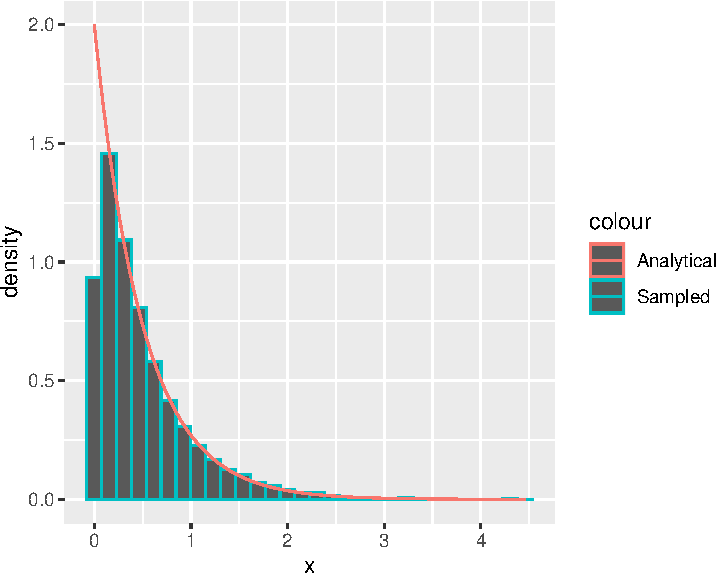
\includegraphics{Project-1_files/figure-latex/unnamed-chunk-1-1} \end{center}

\hypertarget{section-1}{%
\subsection{2}\label{section-1}}

\begin{Shaded}
\begin{Highlighting}[]
\NormalTok{rg }\OtherTok{=} \ControlFlowTok{function}\NormalTok{(n, alpha) \{}
\NormalTok{    u }\OtherTok{=} \FunctionTok{runif}\NormalTok{(}\AttributeTok{n =}\NormalTok{ n)}
\NormalTok{    boundary }\OtherTok{=} \FunctionTok{exp}\NormalTok{(}\DecValTok{1}\NormalTok{)}\SpecialCharTok{/}\NormalTok{(alpha }\SpecialCharTok{+} \FunctionTok{exp}\NormalTok{(}\DecValTok{1}\NormalTok{))}
\NormalTok{    left\_boundary }\OtherTok{=}\NormalTok{ u }\SpecialCharTok{\textless{}}\NormalTok{ boundary}
\NormalTok{    right\_boundary }\OtherTok{=} \SpecialCharTok{!}\NormalTok{left\_boundary}
    
\NormalTok{    u[left\_boundary] }\OtherTok{=}\NormalTok{ (u[left\_boundary]}\SpecialCharTok{/}\NormalTok{boundary)}\SpecialCharTok{\^{}}\NormalTok{(}\DecValTok{1}\SpecialCharTok{/}\NormalTok{alpha)}
\NormalTok{    u[right\_boundary] }\OtherTok{=} \SpecialCharTok{{-}}\FunctionTok{log}\NormalTok{((}\DecValTok{1} \SpecialCharTok{{-}}\NormalTok{ u[right\_boundary])}\SpecialCharTok{/}\NormalTok{(boundary }\SpecialCharTok{*}\NormalTok{ alpha))}
    \FunctionTok{return}\NormalTok{(u)}
\NormalTok{\}}

\NormalTok{dg }\OtherTok{=} \ControlFlowTok{function}\NormalTok{(x, }\AttributeTok{alpha =} \DecValTok{1}\NormalTok{) \{}
\NormalTok{    c }\OtherTok{=}\NormalTok{ alpha }\SpecialCharTok{*} \FunctionTok{exp}\NormalTok{(}\DecValTok{1}\NormalTok{)}\SpecialCharTok{/}\NormalTok{(alpha }\SpecialCharTok{+} \FunctionTok{exp}\NormalTok{(}\DecValTok{1}\NormalTok{))}
\NormalTok{    d }\OtherTok{\textless{}{-}} \FunctionTok{rep}\NormalTok{(}\DecValTok{0}\NormalTok{, }\FunctionTok{length}\NormalTok{(x))}
\NormalTok{    left\_indices }\OtherTok{\textless{}{-}} \DecValTok{0} \SpecialCharTok{\textless{}}\NormalTok{ x }\SpecialCharTok{\&}\NormalTok{ x }\SpecialCharTok{\textless{}} \DecValTok{1}
\NormalTok{    right\_indices }\OtherTok{\textless{}{-}} \DecValTok{1} \SpecialCharTok{\textless{}=}\NormalTok{ x}
\NormalTok{    d[left\_indices] }\OtherTok{\textless{}{-}}\NormalTok{ c }\SpecialCharTok{*}\NormalTok{ (x[left\_indices]}\SpecialCharTok{\^{}}\NormalTok{(alpha }\SpecialCharTok{{-}} \DecValTok{1}\NormalTok{))}
\NormalTok{    d[right\_indices] }\OtherTok{\textless{}{-}}\NormalTok{ c }\SpecialCharTok{*} \FunctionTok{exp}\NormalTok{(}\SpecialCharTok{{-}}\NormalTok{x[right\_indices])}
    \FunctionTok{return}\NormalTok{(d)}
\NormalTok{\}}
\end{Highlighting}
\end{Shaded}

\hypertarget{problem-b}{%
\section{Problem B}\label{problem-b}}

\hypertarget{section-2}{%
\subsection{1}\label{section-2}}

\hypertarget{a}{%
\subsubsection{a)}\label{a}}

We have the gamma distribution constrained to \(\alpha \in (0, 1)\) and
\(\beta = 1\) i.e: \begin{align*}
f(x) = 
\begin{cases}
\frac{1}{\Gamma(\alpha)}x^{\alpha - 1}e^{-x}, \quad 0 < x\\
0, \hspace{48pt} \text{otherwise}
\end{cases}
\end{align*}

Furthermore, we have that \(U \sim \mathrm{unif}(0, 1)\). Thus

\begin{align*}
\text{Acceptance probability} &= P\Big{(}U ≤ \frac{f(x)}{Ag(x)}\Big{)} \\
&= \int_{\mathbb{R}} P\big{(}U ≤ \frac{f(x)}{Ag(x)} \big{|} x\big{)} g(x) dx \\
&= \int_{\mathbb{R}}\frac{f(x)}{Ag(x)}g(x)dx \\
&= \frac{1}{A}\int_{0}^{\infty}f(x)dx = \frac{1}{A}
\end{align*}

Need to find \(A\);
\(Ag(x) ≥ f(x) \, \forall x \Leftrightarrow A ≥ \frac{f(x)}{g(x)}\).
(\(A ≥ 1\), but \(A = 1 \Rightarrow f(x) = g(x)\) and the procedure is
unnecessary) We want A as small as possible. Thus,

\[
A = \sup_{x>0}\frac{f(x)}{g(x)}
\] First we investigate the case when \(0 < x < 1\)

\[
\frac{f(x)}{g(x)}= \frac{\frac{1}{\Gamma(\alpha)}x^{\alpha - 1}e^{-x}} {cx^{\alpha-1}} 
= \frac{e^{-x}}{\Gamma(\alpha)c} 
= \frac{e^{-x}(\alpha^{-1} + e^{-1})}{\Gamma(\alpha)}
\] Supremum provided when \(x \rightarrow 0:\)

\[
\Longrightarrow A = \frac{\alpha^{-1} + e^{-1}}{\Gamma(\alpha)}
\] Now, the case when \(x ≥ 1\): \[
\frac{f(x)}{g(x)} = \frac{\frac{1}{\Gamma(\alpha)}x^{\alpha - 1}e^{-x}} {ce^{-x}} 
= \frac{x^{\alpha-1}}{\Gamma(\alpha)c}
\]

which is maximized for \(x = 1\)

\[
\Longrightarrow A = \frac{\alpha^{-1} + e^{-1}}{\Gamma(\alpha)}
\] same as for \(0 < x < 1\).

\hypertarget{b}{%
\subsubsection{b)}\label{b}}

\begin{Shaded}
\begin{Highlighting}[]
\NormalTok{gamma\_samples }\OtherTok{=} \ControlFlowTok{function}\NormalTok{(}\AttributeTok{n =} \DecValTok{1}\NormalTok{, }\AttributeTok{alpha =} \FloatTok{0.5}\NormalTok{, }\AttributeTok{beta =} \DecValTok{1}\NormalTok{) \{}
    \CommentTok{\# define the acceptance probability}
\NormalTok{    a }\OtherTok{=}\NormalTok{ (}\DecValTok{1}\SpecialCharTok{/}\NormalTok{alpha }\SpecialCharTok{+} \DecValTok{1}\SpecialCharTok{/}\FunctionTok{exp}\NormalTok{(}\DecValTok{1}\NormalTok{))}\SpecialCharTok{/}\FunctionTok{gamma}\NormalTok{(alpha)}
    \CommentTok{\# initialise vector of samples}
\NormalTok{    samples }\OtherTok{=} \FunctionTok{c}\NormalTok{()}
    \CommentTok{\# number of succesful samples}
\NormalTok{    num\_of\_samp }\OtherTok{=} \DecValTok{0}
    \ControlFlowTok{repeat}\NormalTok{ \{}
        \CommentTok{\# Generating n uniform samples on (0, 1)}
\NormalTok{        u }\OtherTok{=} \FunctionTok{runif}\NormalTok{(n)}
        \CommentTok{\# genereate samples from g as in A)}
\NormalTok{        x }\OtherTok{=} \FunctionTok{rg}\NormalTok{(}\AttributeTok{n =}\NormalTok{ n, }\AttributeTok{alpha =}\NormalTok{ alpha)}
        \CommentTok{\# probability of accepting}
\NormalTok{        prob }\OtherTok{=} \FunctionTok{dgamma}\NormalTok{(x, alpha, beta)}\SpecialCharTok{/}\NormalTok{(a }\SpecialCharTok{*} \FunctionTok{dg}\NormalTok{(x, alpha))}
        \CommentTok{\# appending the x{-}s where u \textless{} prob}
\NormalTok{        samples }\OtherTok{=} \FunctionTok{c}\NormalTok{(samples, x[u }\SpecialCharTok{\textless{}}\NormalTok{ prob])}
        \CommentTok{\# increas num\_of\_samp by the number of samples accepted}
\NormalTok{        num\_of\_samp }\OtherTok{=}\NormalTok{ num\_of\_samp }\SpecialCharTok{+} \FunctionTok{length}\NormalTok{(x[u }\SpecialCharTok{\textless{}}\NormalTok{ prob])}
        \CommentTok{\# Here we remove every accepted samples in addition to the n we want}
        \ControlFlowTok{if}\NormalTok{ (}\FunctionTok{length}\NormalTok{(samples) }\SpecialCharTok{\textgreater{}}\NormalTok{ n) \{}
\NormalTok{            samples }\OtherTok{=}\NormalTok{ samples[}\DecValTok{1}\SpecialCharTok{:}\NormalTok{n]}
            \ControlFlowTok{break}
\NormalTok{        \}}
\NormalTok{    \}}
    \FunctionTok{return}\NormalTok{(samples)}
\NormalTok{\}}
\CommentTok{\# We genereate many samples each iteration to save number of iterations in the}
\CommentTok{\# loop. We do this because vector operations are faster than loops, in R.}
\end{Highlighting}
\end{Shaded}

\hypertarget{plotting-an-example-to-comfirm-correct-implementation}{%
\paragraph{Plotting an example to comfirm correct
implementation}\label{plotting-an-example-to-comfirm-correct-implementation}}

\begin{Shaded}
\begin{Highlighting}[]
\NormalTok{alpha }\OtherTok{=} \FloatTok{0.5}
\NormalTok{smpls }\OtherTok{=} \FunctionTok{gamma\_samples}\NormalTok{(}\AttributeTok{n =} \FloatTok{1e+05}\NormalTok{, }\AttributeTok{alpha =}\NormalTok{ alpha)}

\CommentTok{\# sample mean and variance}
\NormalTok{mn }\OtherTok{=} \FunctionTok{mean}\NormalTok{(smpls)}
\NormalTok{vr }\OtherTok{=} \FunctionTok{var}\NormalTok{(smpls)}

\CommentTok{\# to be able to use ggplot we transform the samples to a data frame}
\NormalTok{smpls }\OtherTok{=} \FunctionTok{data.frame}\NormalTok{(}\AttributeTok{samples =}\NormalTok{ smpls)}
\CommentTok{\# making a nice plot for comparison}
\FunctionTok{ggplot}\NormalTok{(}\AttributeTok{data =}\NormalTok{ smpls, }\FunctionTok{aes}\NormalTok{(}\AttributeTok{x =}\NormalTok{ samples)) }\SpecialCharTok{+} \FunctionTok{geom\_histogram}\NormalTok{(}\AttributeTok{data =}\NormalTok{ smpls, }\FunctionTok{aes}\NormalTok{(}\AttributeTok{x =}\NormalTok{ samples, }
    \AttributeTok{y =}\NormalTok{ ..density.., }\AttributeTok{color =} \StringTok{"Sampled"}\NormalTok{)) }\SpecialCharTok{+} \FunctionTok{stat\_function}\NormalTok{(}\AttributeTok{fun =}\NormalTok{ dgamma, }\AttributeTok{geom =} \StringTok{"line"}\NormalTok{, }
    \AttributeTok{size =} \DecValTok{1}\NormalTok{, }\AttributeTok{args =} \FunctionTok{list}\NormalTok{(}\AttributeTok{shape =}\NormalTok{ alpha, }\AttributeTok{rate =} \DecValTok{1}\NormalTok{), }\FunctionTok{aes}\NormalTok{(}\AttributeTok{x =}\NormalTok{ samples, }\AttributeTok{color =} \StringTok{"Analytical"}\NormalTok{)) }\SpecialCharTok{+} 
    \FunctionTok{ylim}\NormalTok{(}\DecValTok{0}\NormalTok{, }\DecValTok{2}\NormalTok{) }\SpecialCharTok{+} \FunctionTok{xlim}\NormalTok{(}\DecValTok{0}\NormalTok{, }\DecValTok{4}\NormalTok{) }\SpecialCharTok{+} \FunctionTok{ggtitle}\NormalTok{(}\StringTok{"Samples and analytical comparison"}\NormalTok{) }\SpecialCharTok{+} \FunctionTok{labs}\NormalTok{(}\AttributeTok{x =} \StringTok{"x"}\NormalTok{, }
    \AttributeTok{y =} \StringTok{"density"}\NormalTok{, }\AttributeTok{caption =} \FunctionTok{paste}\NormalTok{(}\StringTok{"Here we compare the analytical density of f(x) (red line) }\SpecialCharTok{\textbackslash{}n}\StringTok{ with the sampled density (blue bars)."}\NormalTok{)) }\SpecialCharTok{+} 
    \FunctionTok{theme}\NormalTok{(}\AttributeTok{plot.caption =} \FunctionTok{element\_text}\NormalTok{(}\AttributeTok{hjust =} \FloatTok{0.5}\NormalTok{))}
\end{Highlighting}
\end{Shaded}

\begin{center}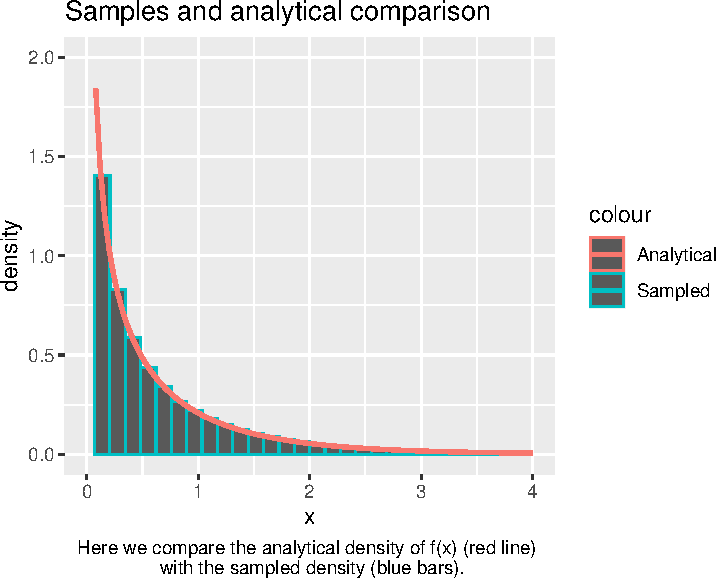
\includegraphics{Project-1_files/figure-latex/unnamed-chunk-4-1} \end{center}

\hypertarget{we-additionally-compare-mean-and-variance}{%
\paragraph{We additionally compare mean and
variance}\label{we-additionally-compare-mean-and-variance}}

\begin{Shaded}
\begin{Highlighting}[]
\NormalTok{beta }\OtherTok{=} \DecValTok{1}
\NormalTok{mean\_var\_matrix }\OtherTok{=} \FunctionTok{matrix}\NormalTok{(}\FunctionTok{c}\NormalTok{(mn, vr, alpha }\SpecialCharTok{*}\NormalTok{ beta, alpha }\SpecialCharTok{*}\NormalTok{ beta}\SpecialCharTok{\^{}}\DecValTok{2}\NormalTok{), }\AttributeTok{ncol =} \DecValTok{2}\NormalTok{, }\AttributeTok{byrow =} \ConstantTok{TRUE}\NormalTok{)}
\FunctionTok{colnames}\NormalTok{(mean\_var\_matrix) }\OtherTok{=} \FunctionTok{c}\NormalTok{(}\StringTok{"Mean"}\NormalTok{, }\StringTok{"Variance"}\NormalTok{)}
\FunctionTok{rownames}\NormalTok{(mean\_var\_matrix) }\OtherTok{=} \FunctionTok{c}\NormalTok{(}\StringTok{"Sample"}\NormalTok{, }\StringTok{"Theoretical"}\NormalTok{)}
\NormalTok{mean\_var\_matrix}
\end{Highlighting}
\end{Shaded}

\begin{verbatim}
##                  Mean  Variance
## Sample      0.4990907 0.4913157
## Theoretical 0.5000000 0.5000000
\end{verbatim}

We can see that the sample mean and variance are fairly similar to that
of the theoretical.

\hypertarget{section-3}{%
\subsection{2}\label{section-3}}

\hypertarget{a-1}{%
\subsubsection{a)}\label{a-1}}

\[
a = \sqrt{\sup_{x} f^{\star}(x)} 
\] For \(x≤0, \; f^{\star}(x) = 0\) thus we examine the case when
\(x>0\): \[
\sup_{x>0}f^{\star}(x) = \sup_{x>0}x^{\alpha-1}e^{-x}
\] Hence, \begin{align*}
\frac{d}{dx}f^{\star}(x) &= (\alpha - 1)x^{\alpha-2}e^{-x} - x^{\alpha-1}e^{-x} \\
&= x^{\alpha-2}e^{-x}((\alpha - 1) - x) = 0 \\
\Longrightarrow x &= \alpha - 1
\end{align*}

moreover

\begin{align*}
\begin{Bmatrix}
f^{\star}(x) \overset{x \rightarrow 0}{\longrightarrow} 0 \\
f^{\star}(x) \overset{x \rightarrow \infty}{\longrightarrow} 0 \\
f^{\star}(\alpha-1) ≥ 0
\end{Bmatrix} 
\overset{f^{\star}(x) \, \text{cont.}}{\Longrightarrow} x = \alpha-1 \; \text{provides a maximum.}
\end{align*}

As a result, \[
a = (\alpha -1)^{(\alpha -1)/2}e^{-(\alpha)+1)/2}
\]

\[
b_+ = \sqrt{\sup_{x≥0}(x^2f^{\star}(x))} 
\] and \[
\sup_{x≥0}(x^2f^{\star}(x)) = x^{\alpha+1}e^{-x} > 0 \; \forall x≥0
\] \begin{align*}
\frac{d}{dx} x^{(\alpha + 1)}e^{-x}
&= (\alpha+1)x^{\alpha}e^{-x} - x^{\alpha+1}e^{-x} \\
&= x^{\alpha}e^{-x}((\alpha + 1) - x) = 0 \\
\Longrightarrow x &= \alpha + 1
\end{align*}

Additionally

\begin{align*}
\begin{Bmatrix}
x^2f^{\star}(x) \overset{x \rightarrow 0}{\longrightarrow} 0 \\
x^2f^{\star}(x) \overset{x \rightarrow \infty}{\longrightarrow} 0
\end{Bmatrix} 
\overset{x^2f^{\star}(x) \, \text{cont.}}{\Longrightarrow} b_+ = (\alpha+1)^{(\alpha+1)/2}e^{-(\alpha+1)/2}
\end{align*}

Furthermore, because \[
f^{\star}(x) \overset{x≤0}{=} 0
\] we get that \[
\quad b_- = -\sqrt{\sup_{x≤0}(x^2f^{\star}(x))} = 0
\]

\hypertarget{b-1}{%
\subsubsection{b)}\label{b-1}}

\begin{Shaded}
\begin{Highlighting}[]
\NormalTok{rum\_gamma }\OtherTok{=} \ControlFlowTok{function}\NormalTok{(}\AttributeTok{n =} \DecValTok{1}\NormalTok{, }\AttributeTok{alpha =} \DecValTok{2}\NormalTok{, }\AttributeTok{beta =} \DecValTok{1}\NormalTok{) \{}
    \CommentTok{\# Calculating the limits of the sample region using the log{-}transformation of a,}
    \CommentTok{\# b\_ and b+}
\NormalTok{    log\_a }\OtherTok{=} \DecValTok{1}\SpecialCharTok{/}\DecValTok{2} \SpecialCharTok{*}\NormalTok{ (alpha }\SpecialCharTok{{-}} \DecValTok{1}\NormalTok{) }\SpecialCharTok{*}\NormalTok{ (}\FunctionTok{log}\NormalTok{(alpha }\SpecialCharTok{{-}} \DecValTok{1}\NormalTok{) }\SpecialCharTok{{-}} \DecValTok{1}\NormalTok{)}
    \CommentTok{\# b\_}
\NormalTok{    b1 }\OtherTok{=} \DecValTok{0}
    \CommentTok{\# log of b\_\{+\}}
\NormalTok{    log\_b2 }\OtherTok{=} \DecValTok{1}\SpecialCharTok{/}\DecValTok{2} \SpecialCharTok{*}\NormalTok{ (alpha }\SpecialCharTok{+} \DecValTok{1}\NormalTok{) }\SpecialCharTok{*}\NormalTok{ (}\FunctionTok{log}\NormalTok{(alpha }\SpecialCharTok{+} \DecValTok{1}\NormalTok{) }\SpecialCharTok{{-}} \DecValTok{1}\NormalTok{)}
    
    \CommentTok{\# creat an empty vector to store samples}
\NormalTok{    samples }\OtherTok{=} \FunctionTok{c}\NormalTok{()}
\NormalTok{    tries }\OtherTok{=} \DecValTok{0}
    \ControlFlowTok{while}\NormalTok{ (}\FunctionTok{length}\NormalTok{(samples) }\SpecialCharTok{\textless{}}\NormalTok{ n) \{}
\NormalTok{        tries }\OtherTok{=}\NormalTok{ tries }\SpecialCharTok{+} \DecValTok{1}
        \CommentTok{\# Sampling from the uniform distribution on (0, 1) and transforming the samples}
        \CommentTok{\# to appropriate regions}
\NormalTok{        log\_y1 }\OtherTok{=}\NormalTok{ log\_a }\SpecialCharTok{+} \FunctionTok{log}\NormalTok{(}\FunctionTok{runif}\NormalTok{(}\DecValTok{1}\NormalTok{))}
\NormalTok{        log\_y2 }\OtherTok{=}\NormalTok{ log\_b2 }\SpecialCharTok{+} \FunctionTok{log}\NormalTok{(}\FunctionTok{runif}\NormalTok{(}\DecValTok{1}\NormalTok{))}
        \ControlFlowTok{if}\NormalTok{ ((alpha }\SpecialCharTok{+} \DecValTok{1}\NormalTok{) }\SpecialCharTok{*}\NormalTok{ log\_y1 }\SpecialCharTok{\textless{}=}\NormalTok{ (alpha }\SpecialCharTok{{-}} \DecValTok{1}\NormalTok{) }\SpecialCharTok{*}\NormalTok{ log\_y2 }\SpecialCharTok{{-}} \FunctionTok{exp}\NormalTok{(log\_y2 }\SpecialCharTok{{-}}\NormalTok{ log\_y1)) \{}
\NormalTok{            y }\OtherTok{=} \FunctionTok{exp}\NormalTok{(log\_y2 }\SpecialCharTok{{-}}\NormalTok{ log\_y1)}
\NormalTok{            samples }\OtherTok{=} \FunctionTok{c}\NormalTok{(samples, y)}
\NormalTok{        \}}
\NormalTok{    \}}
    \FunctionTok{return}\NormalTok{(}\FunctionTok{list}\NormalTok{(}\AttributeTok{tries =}\NormalTok{ tries, }\AttributeTok{samples =}\NormalTok{ samples))}
\NormalTok{\}}
\end{Highlighting}
\end{Shaded}

\hypertarget{plotting-success-rates}{%
\subsubsection{Plotting success rates}\label{plotting-success-rates}}

\begin{Shaded}
\begin{Highlighting}[]
\NormalTok{success\_rates }\OtherTok{=} \ControlFlowTok{function}\NormalTok{(alphas) \{}
\NormalTok{    result }\OtherTok{=} \FunctionTok{c}\NormalTok{()}
\NormalTok{    n }\OtherTok{=} \DecValTok{1000}
    \ControlFlowTok{for}\NormalTok{ (i }\ControlFlowTok{in} \DecValTok{1}\SpecialCharTok{:}\FunctionTok{length}\NormalTok{(alphas)) \{}
        \CommentTok{\# Sample from the algorithm}
\NormalTok{        tries }\OtherTok{=}\NormalTok{ smpls\_rum }\OtherTok{=} \FunctionTok{rum\_gamma}\NormalTok{(}\AttributeTok{n =}\NormalTok{ n, }\AttributeTok{alpha =}\NormalTok{ alphas[i])}\SpecialCharTok{$}\NormalTok{tries}
\NormalTok{        vect }\OtherTok{=} \FunctionTok{c}\NormalTok{(alphas[i], n}\SpecialCharTok{/}\NormalTok{tries)}
\NormalTok{        result }\OtherTok{=} \FunctionTok{cbind}\NormalTok{(result, vect)}
\NormalTok{    \}}
\NormalTok{    result }\OtherTok{=} \FunctionTok{data.frame}\NormalTok{(}\AttributeTok{rates =} \FunctionTok{t}\NormalTok{(result))}
    \FunctionTok{colnames}\NormalTok{(result) }\OtherTok{=} \FunctionTok{c}\NormalTok{(}\StringTok{"Alphas"}\NormalTok{, }\StringTok{"Success\_rates"}\NormalTok{)}
    \FunctionTok{return}\NormalTok{(result)}
\NormalTok{\}}

\NormalTok{small\_alphas }\OtherTok{=} \FunctionTok{c}\NormalTok{(}\DecValTok{2}\NormalTok{, }\DecValTok{5}\NormalTok{, }\DecValTok{10}\NormalTok{, }\DecValTok{20}\NormalTok{, }\DecValTok{30}\NormalTok{, }\DecValTok{40}\NormalTok{, }\DecValTok{50}\NormalTok{)}
\NormalTok{df\_small\_alphas }\OtherTok{=} \FunctionTok{success\_rates}\NormalTok{(small\_alphas)}
\NormalTok{large\_alphas }\OtherTok{=} \FunctionTok{c}\NormalTok{(}\DecValTok{100}\NormalTok{, }\DecValTok{200}\NormalTok{, }\DecValTok{500}\NormalTok{, }\DecValTok{1000}\NormalTok{, }\DecValTok{1500}\NormalTok{, }\DecValTok{2000}\NormalTok{)}
\NormalTok{df\_large\_alphas }\OtherTok{=} \FunctionTok{success\_rates}\NormalTok{(large\_alphas)}


\NormalTok{small }\OtherTok{=} \FunctionTok{ggplot}\NormalTok{(}\AttributeTok{data =}\NormalTok{ df\_small\_alphas) }\SpecialCharTok{+} \FunctionTok{geom\_col}\NormalTok{(}\AttributeTok{data =}\NormalTok{ df\_small\_alphas, }\FunctionTok{aes}\NormalTok{(}\AttributeTok{x =}\NormalTok{ Alphas, }
    \AttributeTok{y =}\NormalTok{ Success\_rates)) }\SpecialCharTok{+} \FunctionTok{labs}\NormalTok{(}\AttributeTok{x =} \StringTok{"Alphas"}\NormalTok{, }\AttributeTok{y =} \StringTok{"Success rates"}\NormalTok{, }\AttributeTok{caption =} \StringTok{"Here we plot the success rates for }\SpecialCharTok{\textbackslash{}n}\StringTok{ alpha = 2, 5, 10, 20, 30, 40 and 50"}\NormalTok{) }\SpecialCharTok{+} 
    \FunctionTok{theme}\NormalTok{(}\AttributeTok{plot.caption =} \FunctionTok{element\_text}\NormalTok{(}\AttributeTok{hjust =} \FloatTok{0.5}\NormalTok{))}

\NormalTok{large }\OtherTok{=} \FunctionTok{ggplot}\NormalTok{(}\AttributeTok{data =}\NormalTok{ df\_large\_alphas) }\SpecialCharTok{+} \FunctionTok{geom\_col}\NormalTok{(}\AttributeTok{data =}\NormalTok{ df\_large\_alphas, }\FunctionTok{aes}\NormalTok{(}\AttributeTok{x =}\NormalTok{ Alphas, }
    \AttributeTok{y =}\NormalTok{ Success\_rates)) }\SpecialCharTok{+} \FunctionTok{labs}\NormalTok{(}\AttributeTok{x =} \StringTok{"Alphas"}\NormalTok{, }\AttributeTok{y =} \StringTok{"Success rates"}\NormalTok{, }\AttributeTok{caption =} \StringTok{"Here we plot the success rates for }\SpecialCharTok{\textbackslash{}n}\StringTok{ alpha = 100, 200, 500, 1000, 1500 and 2000"}\NormalTok{) }\SpecialCharTok{+} 
    \FunctionTok{theme}\NormalTok{(}\AttributeTok{plot.caption =} \FunctionTok{element\_text}\NormalTok{(}\AttributeTok{hjust =} \FloatTok{0.5}\NormalTok{))}


\FunctionTok{grid.arrange}\NormalTok{(small, large, }\AttributeTok{ncol =} \DecValTok{2}\NormalTok{, }\AttributeTok{top =} \StringTok{"Success rates versus alphas, pay attention to the different y{-}axes"}\NormalTok{)}
\end{Highlighting}
\end{Shaded}

\begin{center}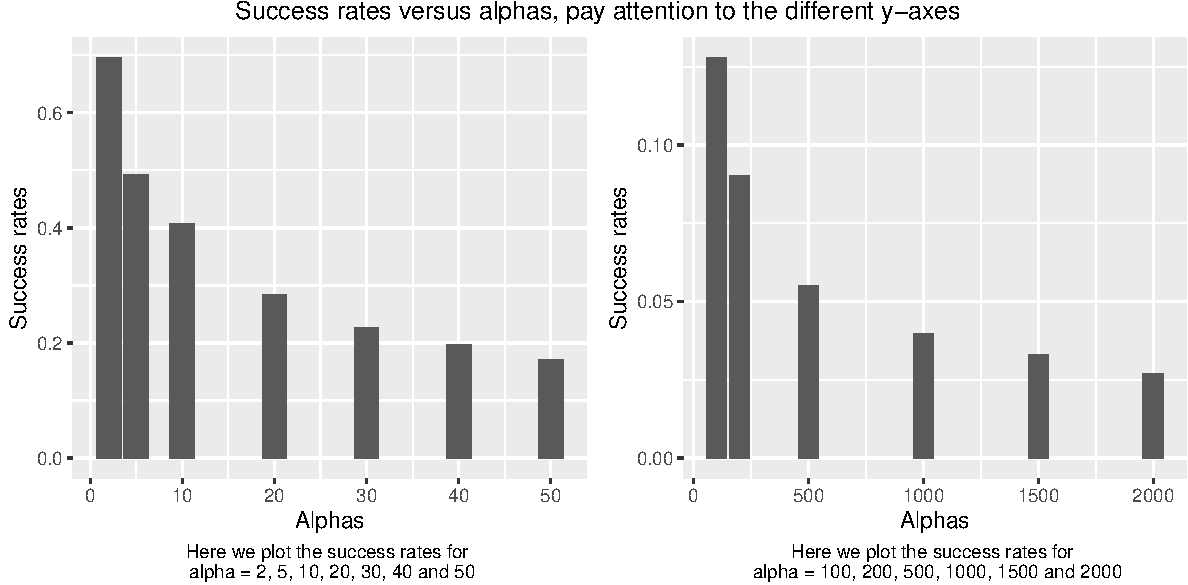
\includegraphics{Project-1_files/figure-latex/unnamed-chunk-7-1} \end{center}

\hypertarget{interpretation}{%
\paragraph{Interpretation}\label{interpretation}}

We see that as \(\alpha\) increases the success rate decreases i.e.~the
algorithm becomes less efficient.

\hypertarget{plotting-one-realisation}{%
\paragraph{Plotting one realisation}\label{plotting-one-realisation}}

We plot one realisation to illustrate that the algorithm works

\begin{Shaded}
\begin{Highlighting}[]
\NormalTok{alpha }\OtherTok{=} \DecValTok{50}
\NormalTok{n }\OtherTok{=} \DecValTok{20000}
\CommentTok{\# Sample from the algorithm}
\NormalTok{smpls\_rum }\OtherTok{=} \FunctionTok{rum\_gamma}\NormalTok{(}\AttributeTok{n =}\NormalTok{ n, }\AttributeTok{alpha =}\NormalTok{ alpha)}
\NormalTok{tries }\OtherTok{=}\NormalTok{ smpls\_rum}\SpecialCharTok{$}\NormalTok{tries}
\NormalTok{samples\_rum }\OtherTok{=}\NormalTok{ smpls\_rum}\SpecialCharTok{$}\NormalTok{samples}
\CommentTok{\# sample mean and variance}
\NormalTok{mn\_rum }\OtherTok{=} \FunctionTok{mean}\NormalTok{(samples\_rum)}
\NormalTok{vr\_rum }\OtherTok{=} \FunctionTok{var}\NormalTok{(samples\_rum)}

\CommentTok{\# to be able to use ggplot we transform the samples to a data frame}
\NormalTok{smpls\_rum }\OtherTok{=} \FunctionTok{data.frame}\NormalTok{(}\AttributeTok{samples =}\NormalTok{ samples\_rum)}

\CommentTok{\# making a nice plot for comparison}
\FunctionTok{ggplot}\NormalTok{(}\AttributeTok{data =}\NormalTok{ smpls\_rum, }\FunctionTok{aes}\NormalTok{(}\AttributeTok{x =}\NormalTok{ samples)) }\SpecialCharTok{+} \FunctionTok{geom\_histogram}\NormalTok{(}\AttributeTok{data =}\NormalTok{ smpls\_rum, }\FunctionTok{aes}\NormalTok{(}\AttributeTok{x =}\NormalTok{ samples, }
    \AttributeTok{y =}\NormalTok{ ..density..), }\AttributeTok{binwidth =} \FloatTok{1.2}\NormalTok{) }\SpecialCharTok{+} \FunctionTok{stat\_function}\NormalTok{(}\AttributeTok{fun =}\NormalTok{ dgamma, }\AttributeTok{geom =} \StringTok{"line"}\NormalTok{, }
    \AttributeTok{size =} \DecValTok{1}\NormalTok{, }\AttributeTok{args =} \FunctionTok{list}\NormalTok{(}\AttributeTok{shape =}\NormalTok{ alpha, }\AttributeTok{rate =} \DecValTok{1}\NormalTok{), }\FunctionTok{aes}\NormalTok{(}\AttributeTok{x =}\NormalTok{ samples))}
\end{Highlighting}
\end{Shaded}

\begin{center}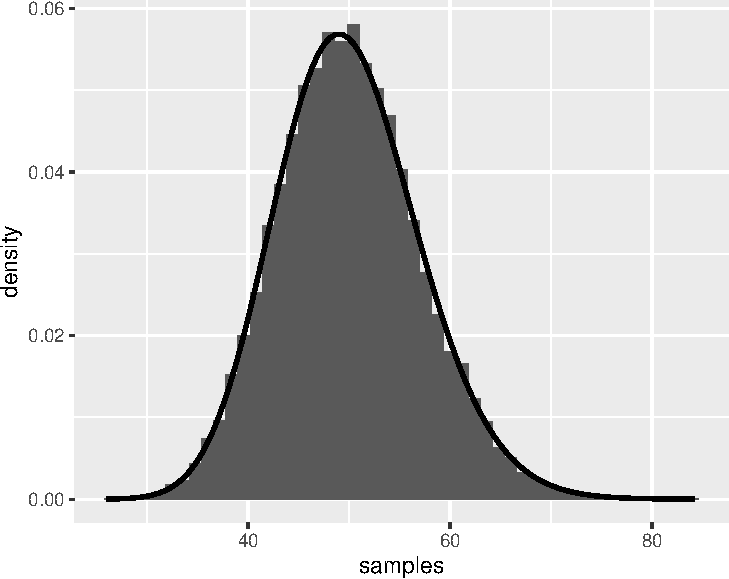
\includegraphics{Project-1_files/figure-latex/unnamed-chunk-8-1} \end{center}

\begin{Shaded}
\begin{Highlighting}[]
\NormalTok{beta }\OtherTok{=} \DecValTok{1}
\NormalTok{mean\_var\_matrix }\OtherTok{=} \FunctionTok{matrix}\NormalTok{(}\FunctionTok{c}\NormalTok{(mn\_rum, vr\_rum, alpha }\SpecialCharTok{*}\NormalTok{ beta, alpha }\SpecialCharTok{*}\NormalTok{ beta}\SpecialCharTok{\^{}}\DecValTok{2}\NormalTok{), }\AttributeTok{ncol =} \DecValTok{2}\NormalTok{, }
    \AttributeTok{byrow =} \ConstantTok{TRUE}\NormalTok{)}
\FunctionTok{colnames}\NormalTok{(mean\_var\_matrix) }\OtherTok{=} \FunctionTok{c}\NormalTok{(}\StringTok{"Mean"}\NormalTok{, }\StringTok{"Var"}\NormalTok{)}
\FunctionTok{rownames}\NormalTok{(mean\_var\_matrix) }\OtherTok{=} \FunctionTok{c}\NormalTok{(}\StringTok{"Sample"}\NormalTok{, }\StringTok{"Theoretical"}\NormalTok{)}
\NormalTok{mean\_var\_matrix}
\end{Highlighting}
\end{Shaded}

\begin{verbatim}
##                 Mean      Var
## Sample      49.97134 49.43265
## Theoretical 50.00000 50.00000
\end{verbatim}

We can see that the sample mean and variance are fairly similar to that
of the theoretical.

\hypertarget{section-4}{%
\subsection{3}\label{section-4}}

For \(X \sim \text{Gamma}(\alpha, 1)\) and \(c \in \mathbb{R}_+\) we get
from the moment generating function that \[
M_{Xc}(t) = E(e^{Xct}) = M_X(ct) = \bigg{(}\frac{1}{1-ct}\bigg{)}^\alpha \\
\Longrightarrow Xc \sim \text{Gamma}(\alpha, c)
\] Thus we can make a simple function using \texttt{rum\_gamma} from
above.

\begin{Shaded}
\begin{Highlighting}[]
\NormalTok{gam4 }\OtherTok{=} \ControlFlowTok{function}\NormalTok{(}\AttributeTok{n =} \DecValTok{1}\NormalTok{, }\AttributeTok{alpha =} \DecValTok{2}\NormalTok{, }\AttributeTok{beta =} \DecValTok{1}\NormalTok{) \{}
    \ControlFlowTok{if}\NormalTok{ (alpha }\SpecialCharTok{\textgreater{}} \DecValTok{1}\NormalTok{) \{}
        \FunctionTok{return}\NormalTok{(beta }\SpecialCharTok{*} \FunctionTok{rum\_gamma}\NormalTok{(n, alpha)}\SpecialCharTok{$}\NormalTok{samples)}
\NormalTok{    \} }\ControlFlowTok{else} \ControlFlowTok{if}\NormalTok{ (alpha }\SpecialCharTok{\textless{}=} \DecValTok{1}\NormalTok{) \{}
        \FunctionTok{return}\NormalTok{(beta }\SpecialCharTok{*} \FunctionTok{gamma\_samples}\NormalTok{(n, alpha))}
\NormalTok{    \}}
\NormalTok{\}}
\end{Highlighting}
\end{Shaded}

\hypertarget{plotting}{%
\paragraph{Plotting}\label{plotting}}

\begin{Shaded}
\begin{Highlighting}[]
\FunctionTok{set.seed}\NormalTok{(}\DecValTok{123}\NormalTok{)}
\NormalTok{n }\OtherTok{=} \DecValTok{10000}
\NormalTok{alpha }\OtherTok{=} \DecValTok{500}
\NormalTok{beta }\OtherTok{=} \DecValTok{5}

\NormalTok{gam4\_realizations }\OtherTok{=} \FunctionTok{gam4}\NormalTok{(n, alpha, beta)}
\CommentTok{\# mean and variance from gam4 samples}
\NormalTok{mn\_gam4 }\OtherTok{=} \FunctionTok{mean}\NormalTok{(gam4\_realizations)}
\NormalTok{vr\_gam4 }\OtherTok{=} \FunctionTok{var}\NormalTok{(gam4\_realizations)}

\NormalTok{gam4\_realizations }\OtherTok{=} \FunctionTok{data.frame}\NormalTok{(}\AttributeTok{samples =}\NormalTok{ gam4\_realizations)}

\FunctionTok{ggplot}\NormalTok{(}\AttributeTok{data =}\NormalTok{ gam4\_realizations, }\FunctionTok{aes}\NormalTok{(}\AttributeTok{x =}\NormalTok{ samples)) }\SpecialCharTok{+} \FunctionTok{geom\_histogram}\NormalTok{(}\AttributeTok{data =}\NormalTok{ gam4\_realizations, }
    \FunctionTok{aes}\NormalTok{(}\AttributeTok{x =}\NormalTok{ samples, }\AttributeTok{y =}\NormalTok{ ..density..)) }\SpecialCharTok{+} \FunctionTok{stat\_function}\NormalTok{(}\AttributeTok{fun =}\NormalTok{ dgamma, }\AttributeTok{geom =} \StringTok{"line"}\NormalTok{, }
    \AttributeTok{size =} \DecValTok{1}\NormalTok{, }\AttributeTok{args =} \FunctionTok{list}\NormalTok{(}\AttributeTok{shape =}\NormalTok{ alpha, }\AttributeTok{rate =} \DecValTok{1}\SpecialCharTok{/}\NormalTok{beta), }\FunctionTok{aes}\NormalTok{(}\AttributeTok{x =}\NormalTok{ samples))}
\end{Highlighting}
\end{Shaded}

\begin{center}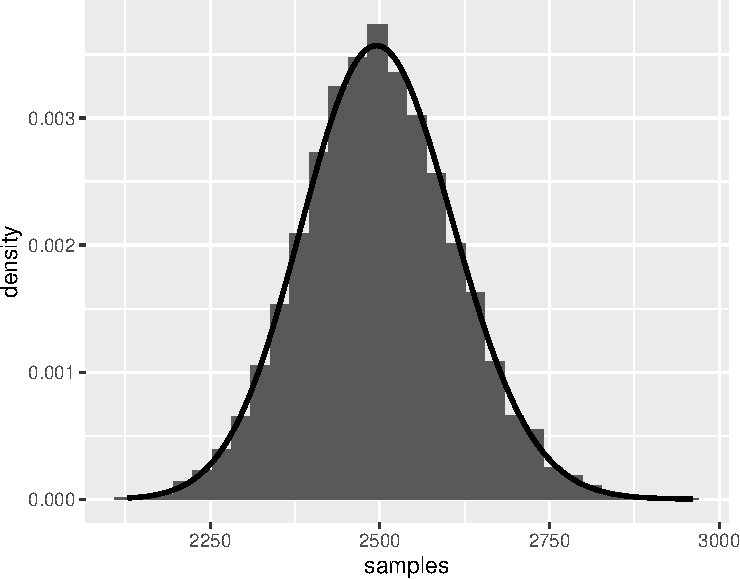
\includegraphics{Project-1_files/figure-latex/unnamed-chunk-11-1} \end{center}

\hypertarget{comparing-mean-and-variance}{%
\paragraph{Comparing mean and
variance}\label{comparing-mean-and-variance}}

\begin{Shaded}
\begin{Highlighting}[]
\NormalTok{mean\_var\_matrix }\OtherTok{=} \FunctionTok{matrix}\NormalTok{(}\FunctionTok{c}\NormalTok{(mn\_gam4, vr\_gam4, alpha }\SpecialCharTok{*}\NormalTok{ beta, alpha }\SpecialCharTok{*}\NormalTok{ beta}\SpecialCharTok{\^{}}\DecValTok{2}\NormalTok{), }\AttributeTok{ncol =} \DecValTok{2}\NormalTok{, }
    \AttributeTok{byrow =} \ConstantTok{TRUE}\NormalTok{)}
\FunctionTok{colnames}\NormalTok{(mean\_var\_matrix) }\OtherTok{=} \FunctionTok{c}\NormalTok{(}\StringTok{"Mean"}\NormalTok{, }\StringTok{"Var"}\NormalTok{)}
\FunctionTok{rownames}\NormalTok{(mean\_var\_matrix) }\OtherTok{=} \FunctionTok{c}\NormalTok{(}\StringTok{"Sample"}\NormalTok{, }\StringTok{"Theoretical"}\NormalTok{)}
\NormalTok{mean\_var\_matrix}
\end{Highlighting}
\end{Shaded}

\begin{verbatim}
##                 Mean     Var
## Sample      2499.001 12547.5
## Theoretical 2500.000 12500.0
\end{verbatim}

\hypertarget{section-5}{%
\subsection{4}\label{section-5}}

\hypertarget{a-2}{%
\subsubsection{a)}\label{a-2}}

\[
X \sim \text{Gamma}(\alpha, 1) \\
Y \sim \text{Gamma}(\beta, 1)
\] are independent and from above we have learned that \[
X+Y = V \sim \text{Gamma}(\alpha + \beta, 1).
\] The joint pdf of \(X\) and \(Y\) is \[
f_{X, Y}(x, y) = \frac{1}{\Gamma(\alpha)\Gamma(\beta)}x^{\alpha-1}y^{\beta-1}e^{-(x+y)}, \quad x,y ≥ 0
\] We further define \[
U = \frac{X}{X + Y} = \frac{X}{V}
\] Then \[
X = UV ≥0 \quad \text{and} \quad Y = V-X = V-UV = V(1-U) ≥0
\] Hence we have two cases

\begin{enumerate}
\def\labelenumi{\arabic{enumi}.}
\tightlist
\item
  \(V ≥ 0 \Rightarrow 0 ≤ U ≤ 1\)
\item
  \(V < 0 \Rightarrow U ≤ 0\) and \(U ≥ 1\) (Which clearly is not
  possible)
\end{enumerate}

Now we find the determinant of the Jacobian of the transformation

\[
|J| = \Bigg|\frac{\partial(X,Y)}{\partial(U, V)}\Bigg| 
= \begin{vmatrix}
V & U \\
-V & 1-V
\end{vmatrix} = V - UV + UV = V
\] Hence, we get

\begin{align*}
f_{U, V}(u, v) &= \frac{1}{\Gamma(\alpha)\Gamma(\beta)}(uv)^{\alpha-1}v(1-u))^{\beta-1}e^{-v} \Bigg|\frac{\partial(x, y)}{\partial(u, v)}\Bigg| \\
&= \frac{1}{\Gamma(\alpha)\Gamma(\beta)}v^{\alpha-1+\beta-1+1} u^{\alpha-1}(1-u)^{\beta-1}e^{-v} \\
&= \frac{1}{\Gamma(\alpha)\Gamma(\beta)}v^{\alpha+\beta-1}e^{-v} u^{\alpha-1}(1-u)^{\beta-1} \frac{\Gamma(\alpha + \beta)}{\Gamma(\alpha + \beta)} \\
&= \underline{\frac{1}{\Gamma(\alpha + \beta)}v^{(\alpha + \beta) - 1}e^{-v}} \;
\underline{\frac{\Gamma(\alpha + \beta)}{\Gamma(\alpha)\Gamma(\beta)} u^{\alpha-1}(1-u)^{\beta-1}}
\end{align*}

We define the first part of the expression as \(f_V(v)\) which we
identify to be tha Gamma density with variables \(\alpha + \beta\) and
\(1\). Furthermore, the last part we define as \(f_U(u)\) and see that
it is the pdf of a Beta distributed variables \(\alpha\) and \(\beta\).
Since these pdfs are entirely seperated can conclude that \[
U \sim \text{Beta}(\alpha, \beta) \quad \blacksquare
\]

\hypertarget{b-2}{%
\subsubsection{b)}\label{b-2}}

\begin{Shaded}
\begin{Highlighting}[]
\NormalTok{beta\_gen }\OtherTok{=} \ControlFlowTok{function}\NormalTok{(n, alpha, beta) \{}
\NormalTok{    x }\OtherTok{=} \FunctionTok{rum\_gamma}\NormalTok{(n, alpha)}\SpecialCharTok{$}\NormalTok{samples}
\NormalTok{    y }\OtherTok{=} \FunctionTok{rum\_gamma}\NormalTok{(n, beta)}\SpecialCharTok{$}\NormalTok{samples}
    \FunctionTok{return}\NormalTok{(x}\SpecialCharTok{/}\NormalTok{(x }\SpecialCharTok{+}\NormalTok{ y))}
\NormalTok{\}}
\end{Highlighting}
\end{Shaded}

\hypertarget{plotting-1}{%
\paragraph{Plotting}\label{plotting-1}}

\begin{Shaded}
\begin{Highlighting}[]
\NormalTok{n }\OtherTok{=} \DecValTok{20000}
\NormalTok{alpha }\OtherTok{=} \DecValTok{5}
\NormalTok{beta }\OtherTok{=} \DecValTok{2}
\NormalTok{beta\_vect }\OtherTok{=} \FunctionTok{beta\_gen}\NormalTok{(n, alpha, beta)}
\CommentTok{\# Sample mean and variance}
\NormalTok{mn\_beta }\OtherTok{=} \FunctionTok{mean}\NormalTok{(beta\_vect)}
\NormalTok{vr\_beta }\OtherTok{=} \FunctionTok{var}\NormalTok{(beta\_vect)}

\NormalTok{beta\_vect }\OtherTok{=} \FunctionTok{data.frame}\NormalTok{(}\AttributeTok{samples =}\NormalTok{ beta\_vect)}
\CommentTok{\# Plot}
\FunctionTok{ggplot}\NormalTok{(}\AttributeTok{data =}\NormalTok{ beta\_vect, }\FunctionTok{aes}\NormalTok{(}\AttributeTok{x =}\NormalTok{ samples)) }\SpecialCharTok{+} \FunctionTok{geom\_histogram}\NormalTok{(}\AttributeTok{data =}\NormalTok{ beta\_vect, }\FunctionTok{aes}\NormalTok{(}\AttributeTok{x =}\NormalTok{ samples, }
    \AttributeTok{y =}\NormalTok{ ..density..)) }\SpecialCharTok{+} \FunctionTok{stat\_function}\NormalTok{(}\AttributeTok{fun =}\NormalTok{ dbeta, }\AttributeTok{geom =} \StringTok{"line"}\NormalTok{, }\AttributeTok{size =} \DecValTok{1}\NormalTok{, }\AttributeTok{args =} \FunctionTok{list}\NormalTok{(}\AttributeTok{shape1 =}\NormalTok{ alpha, }
    \AttributeTok{shape2 =}\NormalTok{ beta), }\FunctionTok{aes}\NormalTok{(}\AttributeTok{x =}\NormalTok{ samples))}
\end{Highlighting}
\end{Shaded}

\begin{center}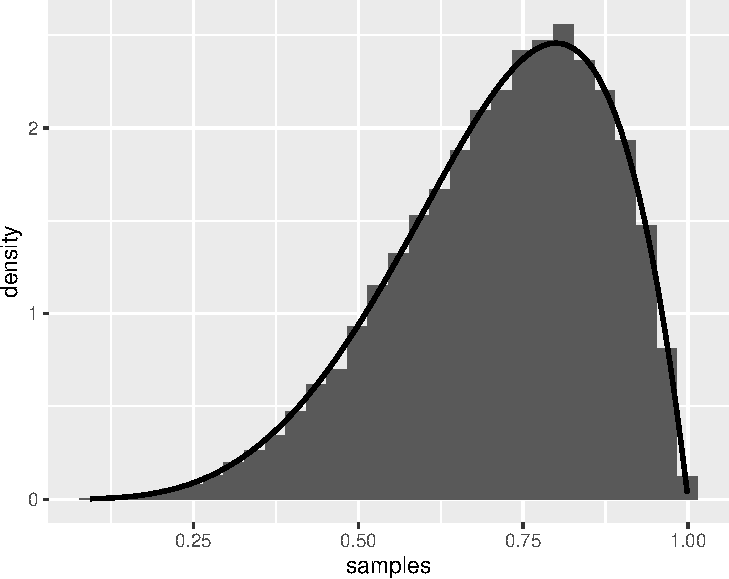
\includegraphics{Project-1_files/figure-latex/unnamed-chunk-14-1} \end{center}

\hypertarget{comparing-mean-and-variance-1}{%
\paragraph{Comparing mean and
variance}\label{comparing-mean-and-variance-1}}

\begin{Shaded}
\begin{Highlighting}[]
\NormalTok{mean\_var\_matrix }\OtherTok{=} \FunctionTok{matrix}\NormalTok{(}\FunctionTok{c}\NormalTok{(mn\_beta, vr\_beta, alpha}\SpecialCharTok{/}\NormalTok{(alpha }\SpecialCharTok{+}\NormalTok{ beta), alpha }\SpecialCharTok{*}\NormalTok{ beta}\SpecialCharTok{/}\NormalTok{((alpha }\SpecialCharTok{+} 
\NormalTok{    beta)}\SpecialCharTok{\^{}}\DecValTok{2} \SpecialCharTok{*}\NormalTok{ (alpha }\SpecialCharTok{+}\NormalTok{ beta }\SpecialCharTok{+} \DecValTok{1}\NormalTok{))), }\AttributeTok{ncol =} \DecValTok{2}\NormalTok{, }\AttributeTok{byrow =} \ConstantTok{TRUE}\NormalTok{)}
\FunctionTok{colnames}\NormalTok{(mean\_var\_matrix) }\OtherTok{=} \FunctionTok{c}\NormalTok{(}\StringTok{"Mean"}\NormalTok{, }\StringTok{"Var"}\NormalTok{)}
\FunctionTok{rownames}\NormalTok{(mean\_var\_matrix) }\OtherTok{=} \FunctionTok{c}\NormalTok{(}\StringTok{"Sample"}\NormalTok{, }\StringTok{"Theoretical"}\NormalTok{)}
\NormalTok{mean\_var\_matrix}
\end{Highlighting}
\end{Shaded}

\begin{verbatim}
##                  Mean        Var
## Sample      0.7153356 0.02517216
## Theoretical 0.7142857 0.02551020
\end{verbatim}

We can see that the sample mean and variance are fairly similar to that
of the theoretical.

\end{document}
